\documentclass{beamer}
\usetheme{metropolis}           % Use metropolis theme
\title{On Proportional Symbol Maps - An applied perspective}
\date{\today}
\author{David Gödecke, Philip Mayer, Roland Siegbert}
\institute{Geometry Lab SS 2020}


\usepackage{xcolor}
\newcommand{\red}{\textcolor{red}}
\newcommand{\blue}{\textcolor{blue}}

\begin{document}

  \maketitle

  \begin{frame}{Overview - ToC}
    \tableofcontents
  \end{frame}

  \section{Introduction}

  \begin{frame}{Motivation}
    A few words on why.
    Picture of COVID-19 and similar data.
  \end{frame}

  \begin{frame}{Proportional Symbol Maps}
    Backreference.
    Explanation of topic.
  \end{frame}

  \begin{frame}{Maps and Glyphs}
    Introduce glyph types discussed and create transition into Algo section.
  \end{frame}

  \section{Algorithms}

  \begin{frame}{Prior}
    David's part. See Philip's list and or discussion.
  \end{frame}

  \begin{frame}{Generalized}
    See Philip's list and or discussion.
  \end{frame}

  \begin{frame}{Our approach}
    See Philip's list and or discussion.
  \end{frame}

  \begin{frame}{Squares and Pies... and so on}
    See Philip's list and or discussion.
  \end{frame}

  \section{Experimental results}

  \begin{frame}{Experimental Setup}
	\begin{itemize}
		\item We use the John Hopkins University Covid-19 data
		\item recovered cases are colored green, deceased cases are colored black and 		the infected are colored red
		\item logarithmic scaling dependent on two parameters:
		\begin{align*}
			r=M* \log \left( \frac{c_i S}{c_{max}} \right)
		\end{align*}
		$M$ is the maximum size of a glyph, $S$ is a scaling factor and $c_{max}$ is 			the maximum number of cases
	\end{itemize}
\end{frame}
  
  
  
  \begin{frame}
\begin{figure}[!t]
  \centering
  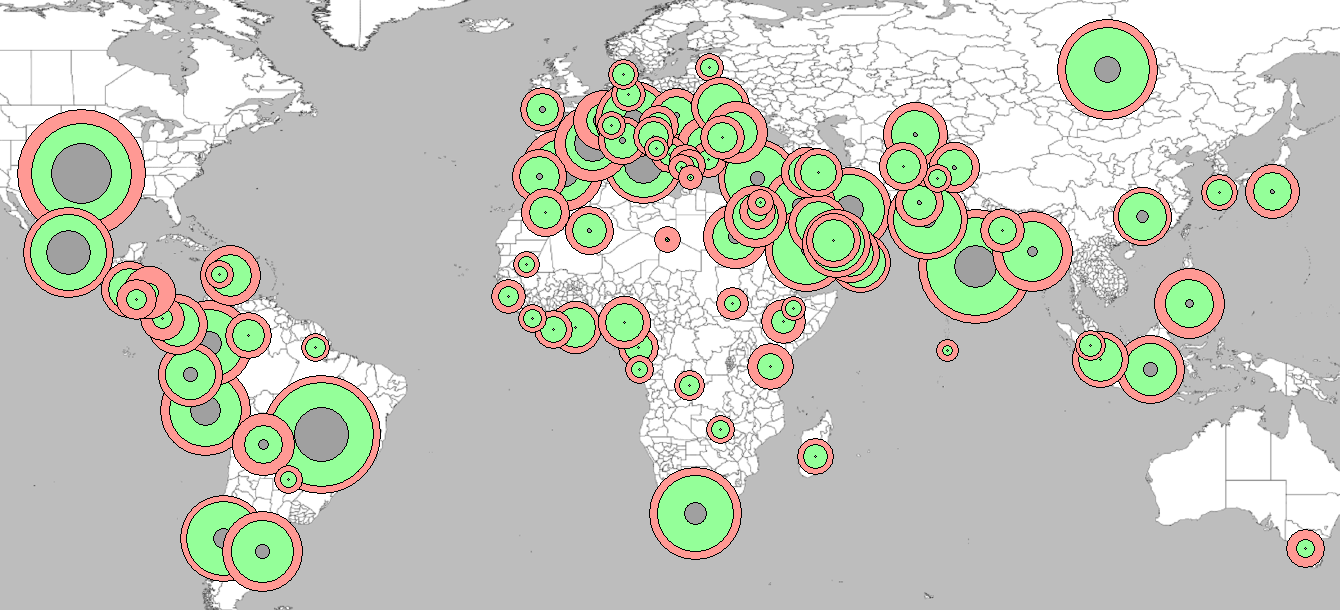
\includegraphics[height=5cm]{MinMinAbsEval.png}
\end{figure}

\begin{table}
\resizebox{9cm}{!}{%
    \begin{tabular}{| l || p{1.3cm} | p{1.7cm} | p{1.7cm} | p{1.5cm} | p{1.5cm} | p{1.5cm} |}
      \hline
      algorithm            & covered & minVis (rel) & minVis (abs) & min one glyph & average rel vis & absolute perc \\
      \hline
      random               &  \blue{44}      & 0.071 (0)    & 0.995 (0)    & 0             & 0.658           & 0.677         \\

      LeftToRight          & \blue {42}      & 0.331 (0)    & 2.189 (0)    & 0             & 0.641           & 0.678         \\

      RightToLeft          &\blue {  43}      & 0.324 (0)    & 0.995 (0)    & 0             & 0.656           & 0.693         \\
	\hline
      Painter              &\blue {  16 }     & 0.408 (0)    & 6.283 (0)    & 34.991        & 0.761           & 0.718    
     \\

      MinMinStacking (abs) &\blue {  16 }     & 0.473 (0)    & 2.189 (0)    & 44.467        & 0.757           & 0.724         \\
      
      \hline
      MinMinStacking (rel) &\blue { 18 }     & 0.691 (0)    & 2.189 (0)    & 37.327        & 0.748           & 0.725         \\

      MinSumStacking (abs) &\blue { 18}      & 0.702 (0)    & 3.974 (0)    & \red{44.467}        & 0.75            & 0.721         \\

      MinSumStacking (rel) &\blue {  18 }     & 0.702 (0)    & 2.189 (0)    & 37.327        & 0.744           & 0.723         \\

      \hline
    \end{tabular}}
\caption{date: 02.08.2020  , parameters: $M=50$, $S=500$ and $\text{minimum number of cases}=5000$  }
\end{table}
\end{frame}

\begin{frame}
\begin{figure}[!t]
  \centering
  \includegraphics[height=5cm]{HawaiianEval}
\end{figure}
\begin{table}[!h]
\begin{center}
\resizebox{9cm}{!}{%
    \begin{tabular}{| l || p{1.3cm} | p{1.7cm} | p{1.7cm} | p{1.5cm} | p{1.5cm} | p{1.5cm} |}
      \hline
      algorithm    & covered & minVis (rel) & minVis (abs) & min one Glyph & average rel vis & absolute perc \\
      \hline
      random       & 21      & 0.025 (0)    & 0.589 (0)    & 0             & 0.765           & 0.714         \\

      LeftToRight  & 12      & 0.948 (0)    & 2.743 (0)    & 0             & 0.775           & 0.725         \\

      RightToLeft  & 13      & 0.664 (0)    & 2.89 (0)     & 0             & 0.783           & 0.735         \\
\hline
      Painter      & \red 0       & 0.585        & 6.283        & 47.758        & 0.857           & 0.759         \\

      our Stacking & \red 0       & 2.342        & 6.283        & 75.034        & 0.859           & 0.77          \\

      \hline
    \end{tabular}}
  \end{center}
  \caption{date: 02.08.2020  , $M=50$, $S=500$ and $\text{MnC}=5000$  }
\end{table}
\end{frame}

\begin{frame}
\begin{table}
\resizebox{9cm}{!}{%
    \begin{tabular}{| l || p{1.3cm} | p{1.7cm} | p{1.7cm} | p{1.5cm} | p{1.5cm} | p{1.5cm} |}
      \hline
      algorithm            & covered & minVis (rel) & minVis (abs) & min one glyph & average rel vis & absolute perc \\
      \hline
      random               & 44      & 0.071 (0)    & 0.995 (0)    & 0             & 0.658           & 0.677         \\

      LeftToRight          & 42      & 0.331 (0)    & 2.189 (0)    & 0             & 0.641           & 0.678         \\

      RightToLeft          & 43      & 0.324 (0)    & 0.995 (0)    & 0             & 0.656           & 0.693         \\
\hline
      Painter              & 16      & 0.408 (0)    & 6.283 (0)    & 34.991        & \red {0.761}           & \red {0.718}         \\

      MinMinStacking (abs) & 16      & 0.473 (0)    & 2.189 (0)    & 44.467        & \red {0.757}           & \red {0.724}         \\
\hline
      MinMinStacking (rel) & 18      & 0.691 (0)    & 2.189 (0)    & 37.327        & 0.748           & 0.725         \\

      MinSumStacking (abs) & 18      & 0.702 (0)    & 3.974 (0)    & 44.467        & 0.75            & 0.721         \\

      MinSumStacking (rel) & 18      & 0.702 (0)    & 2.189 (0)    & 37.327        & 0.744           & 0.723         \\

      \hline
    \end{tabular}}
\caption{centered disks  }
\end{table}

\begin{table}[!h]
  \begin{table}[!h]
\begin{center}
\resizebox{9cm}{!}{%
    \begin{tabular}{| l || p{1.3cm} | p{1.7cm} | p{1.7cm} | p{1.5cm} | p{1.5cm} | p{1.5cm} |}
      \hline
      algorithm    & covered & minVis (rel) & minVis (abs) & min one Glyph & average rel vis & absolute perc \\
      \hline
      random       & 21      & 0.025 (0)    & 0.589 (0)    & 0             & 0.765           & 0.714         \\

      LeftToRight  & 12      & 0.948 (0)    & 2.743 (0)    & 0             & 0.775           & 0.725         \\

      RightToLeft  & 13      & 0.664 (0)    & 2.89 (0)     & 0             & 0.783           & 0.735         \\
\hline
      Painter      &\red 0       & 0.585        & 6.283        & 47.758        & 0.857           & 0.759         \\

      our Stacking &\red 0       & 2.342        & 6.283        & 75.034        & 0.859           & 0.77          \\

      \hline
    \end{tabular}}
  \end{center}
 \caption{
  date: 02.08.2020  , $M=50$, $S=500$ and $\text{MnC}=5000$ }
\end{table}
\end{table}

\end{frame}

\begin{frame}
\begin{figure}[!t]
  \centering
  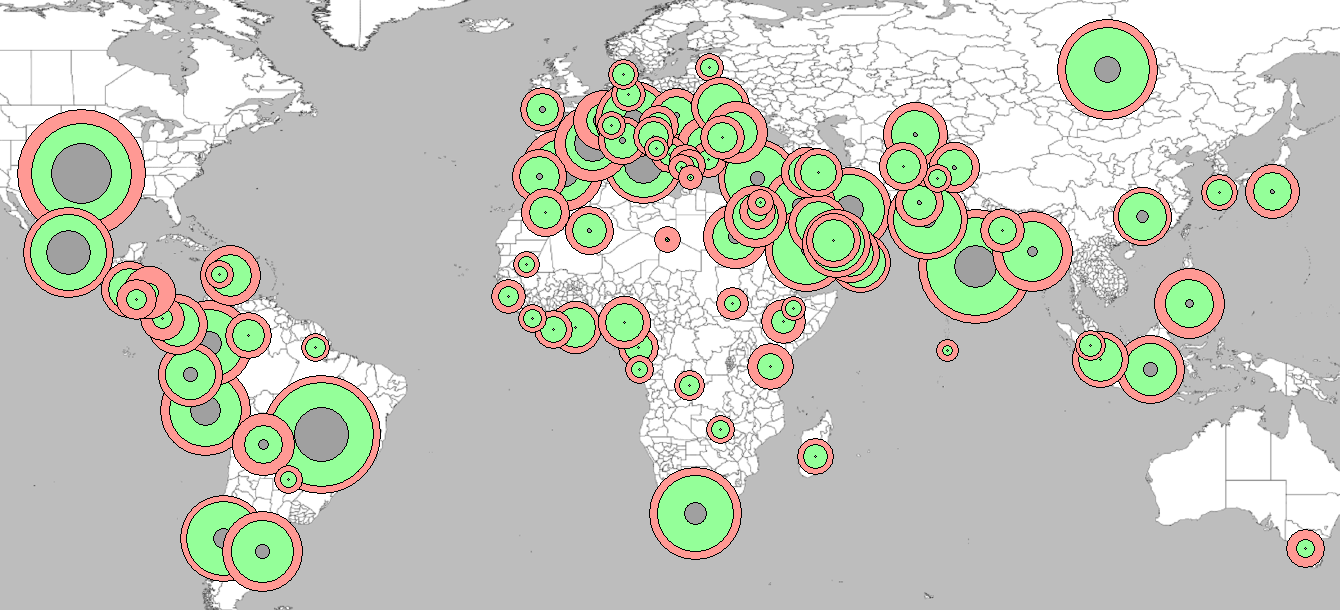
\includegraphics[height=4cm]{MinMinAbsEval.png}
\end{figure}
\begin{figure}[!t]
  \centering
  \includegraphics[height=4cm]{HawaiianEval}
\end{figure}



\end{frame}
\begin{frame}

\begin{figure}[!b]
  \centering
  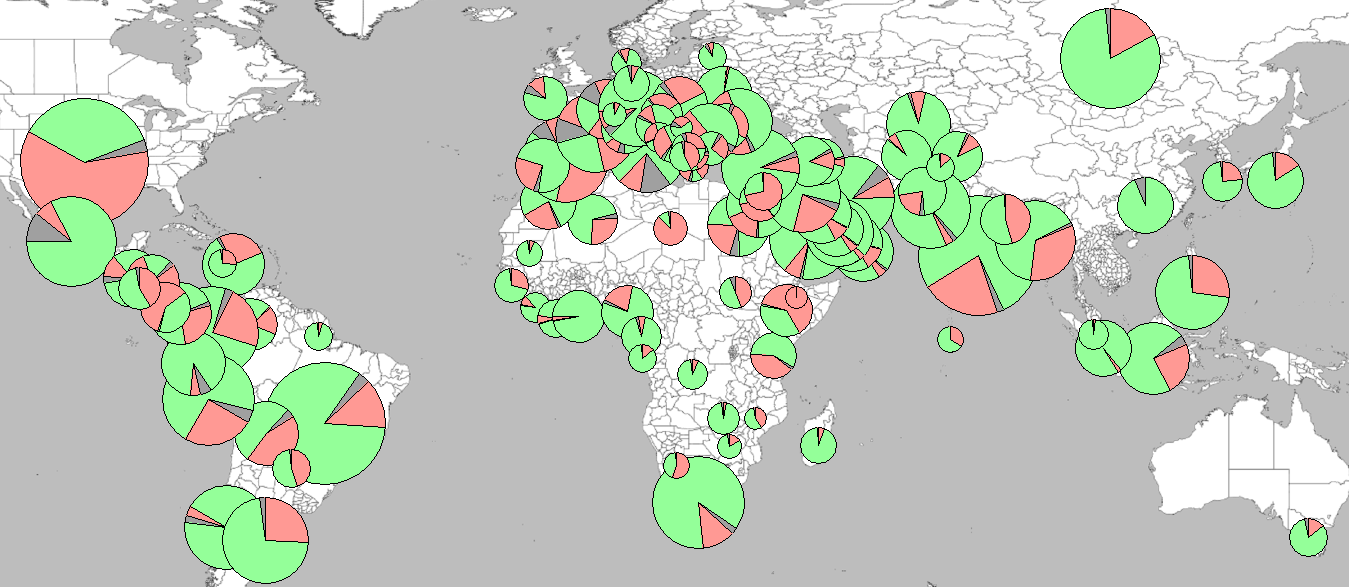
\includegraphics[height=5cm]{pieChartsEval}
\end{figure}

\begin{table}[h]
  \begin{center}
  \resizebox{9cm}{!}{
    \begin{tabular}{| l || l | l | l | l |}
      \hline
      algorithm          & covered & minDist   & minDistAvg & maxDistAvg \\
      \hline
      Painter+random     & \red {60}     & 0.002 (0) & 1.211       & 4.035      \\

      random+heuristic   & 24      & 0.0 (0)   & 1.687      & 2.573      \\

      RightToLeft        & 18      & 0.017 (0) & 1.719      & 2.685      \\
\hline
      Painter+ heuristic & \red 6       & 0.022 (0) & 1.733      & 2.648      \\

      our Stacking       & \red 0       & 0.271     & 1.765      & 2.838      \\

      \hline
    \end{tabular}}
  \end{center}
  \caption{date: 22.08.2020  , $M=50$, $S=500$ and $\text{MnC}=5000$  }
\end{table}
\end{frame}


\begin{frame}

\begin{figure}[b]
  \centering
  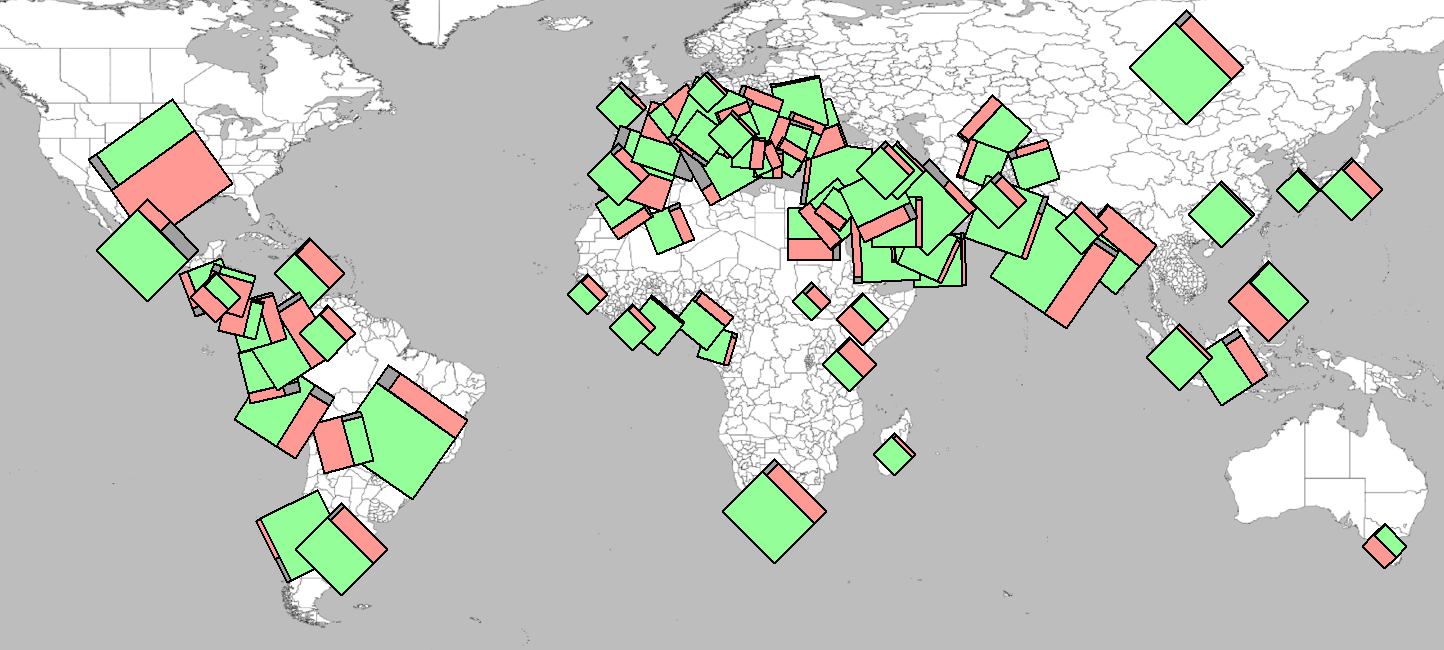
\includegraphics[height=5cm]{squaresEval}

\end{figure}

\begin{table}[h]
  \begin{center}
  \resizebox{7cm}{!}{
    \begin{tabular}{| l || l | l | }
      \hline
      algorithm                           & covered & minDist \\  %& minDistAvg \\
      \hline

      random Stacking+random rotations    & 35      & 0.361 (0)\\ %& 35.846     \\

      Painter+random rotations            & 17      & 0.251 (0)\\ %& 34.406     \\

      random Stacking+heuristic rotations & 26      & 0.038 (0)\\ %& 34.776     \\
\hline
      Painter+heuristic                   & \red{14}      & 0.263 (0)\\ %& 32.061     \\

      our Stacking                        & \red 7       & 0.078 (0)\\ %& 25.232     \\

      \hline
    \end{tabular}}
  \end{center}
  \caption{
    date: 22.08.2020  , $M=50$, $S=500$ and $\text{MnC}=5000$  }

\end{table}

\end{frame}

\begin{frame}
\begin{figure}[!b]
  \centering
  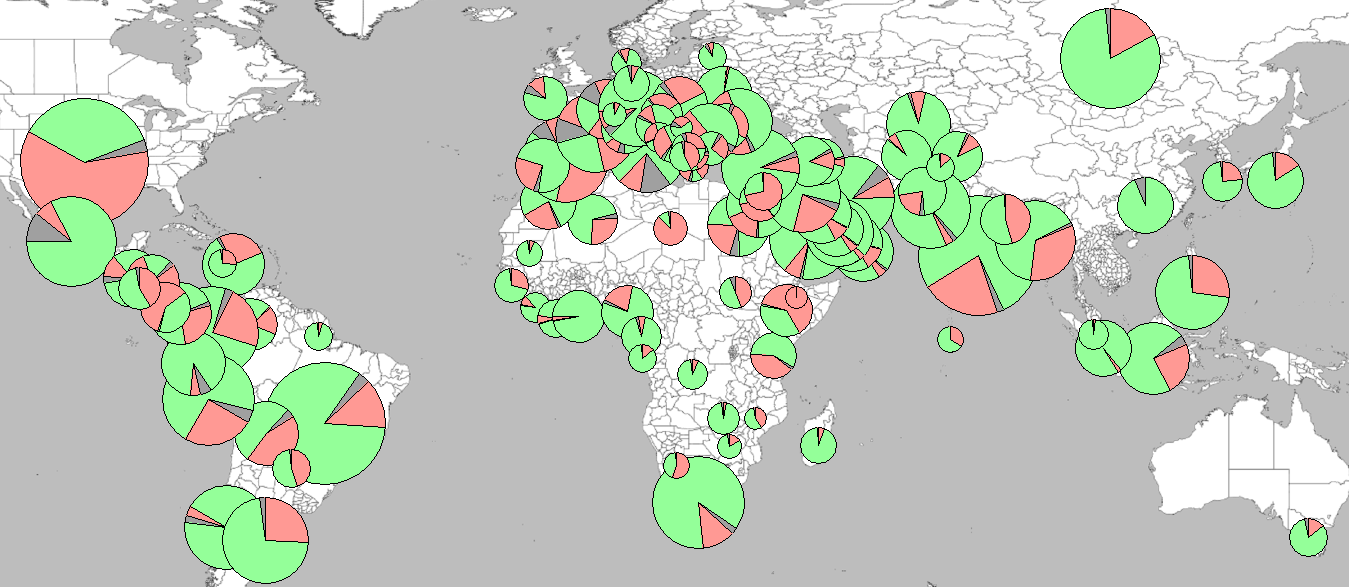
\includegraphics[height=4.2cm]{pieChartsEval}
\end{figure}

\begin{figure}[b]
  \centering
  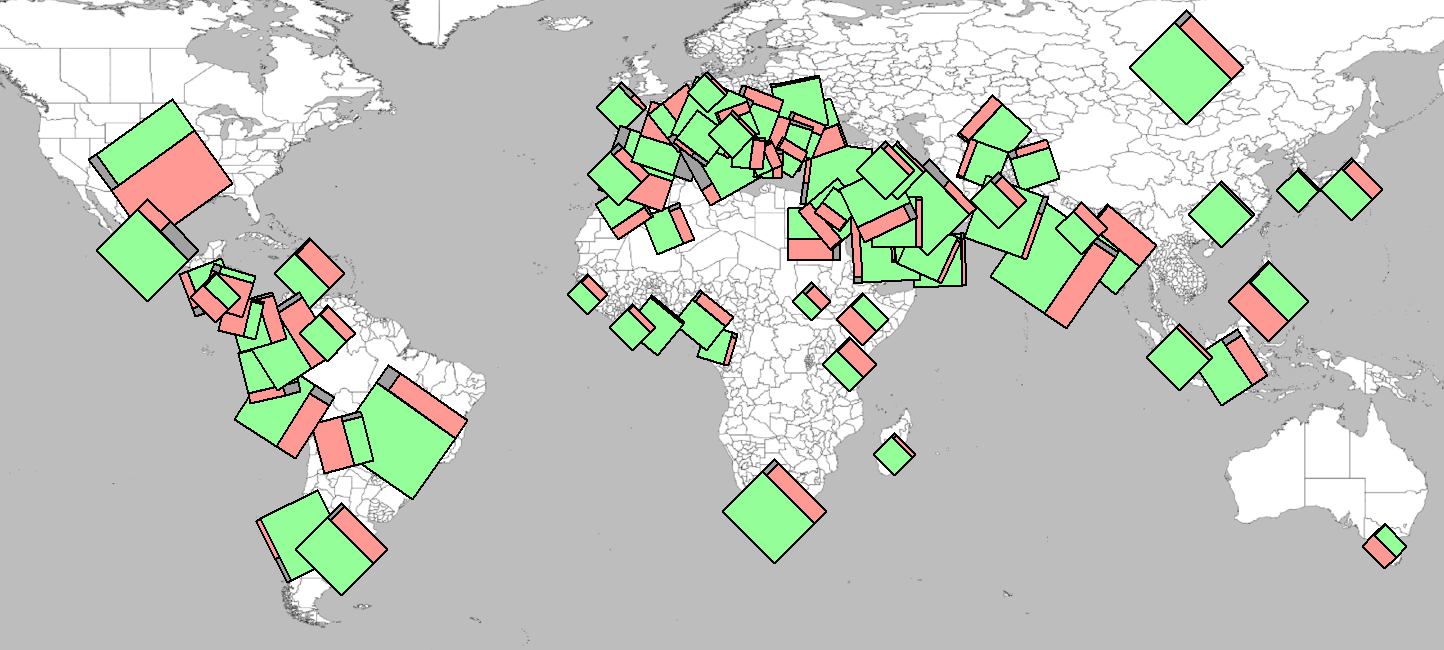
\includegraphics[height=4.2cm]{squaresEval}

\end{figure}


\end{frame}



  \section{Exploration in App}

  \begin{frame}{Exploration of the data}
    [Switch to app and play!]
  \end{frame}

  \section{Conclusion and Outlook}

  \begin{frame}{Summary}

    \begin{itemize}
      \item Four glyphs were shown, with two new approaches.
      \item NP-hardness of new approaches was outlined.
      \item Heuristics and greedy approach usually are good choices.
      \item Square/pie approach can be interpreted as discrete version of the relative visibility.
      \item All of this was verified on the most recent COVID-19 data,
      \item and experimentally demonstrated.
    \end{itemize}
  \end{frame}

\end{document}
